SSD和YOLO一样都是采用一个CNN网络来进行检测,但是却采用了多尺度的特征图,其基本架构如图\ref{ssd}所示。
\begin{uscfigure}
	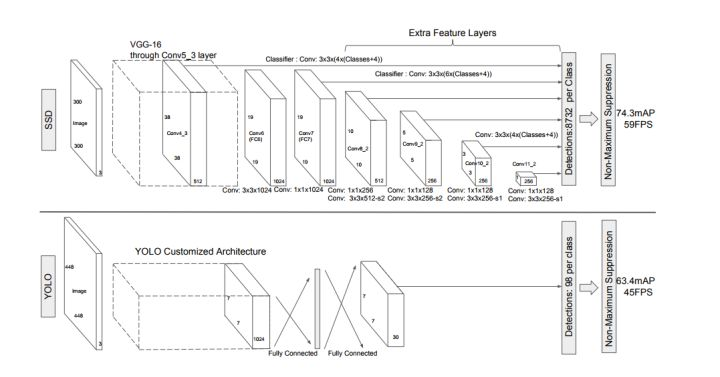
\includegraphics[width=\textwidth]{./Pictures/ssd_modual.jpg}	
	\caption{SSD基本框架}
	\label{ssd}
\end{uscfigure}


下面将SSD核心设计思想总结为以下三点:

\textbf{1、采用多尺度特征图用于检测 }

所谓多尺度采用大小不同的特征图,CNN网络一般前面的特征图比较大,后面会逐渐采用stride=2的卷积或者pool来降低特征图大小,如图\ref{multiscale}所示
\begin{uscfigure}
	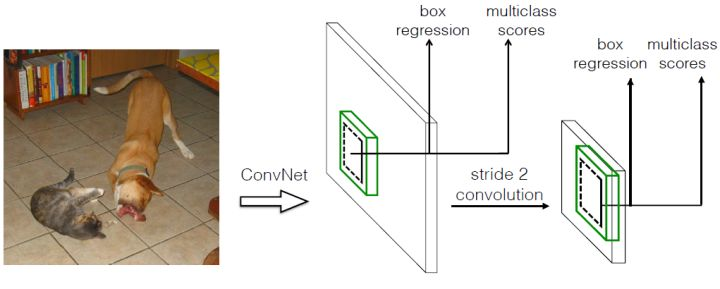
\includegraphics[width=\textwidth]{./Pictures/ssd_(1).jpg}	
	\caption{采用多尺度用于检测}
	\label{multiscale}
\end{uscfigure}
一个比较大的特征图和一个比较小的特征图,它们都用来做检测。这样做的好处是比较大的特征图来用来检测相对较小的目标,而小的特征图负责检测大目标,如图\ref{featuremap}所示,8x8的特征图可以划分更多的单元,但是其每个单元的先验框尺度比较小。
\begin{uscfigure}
	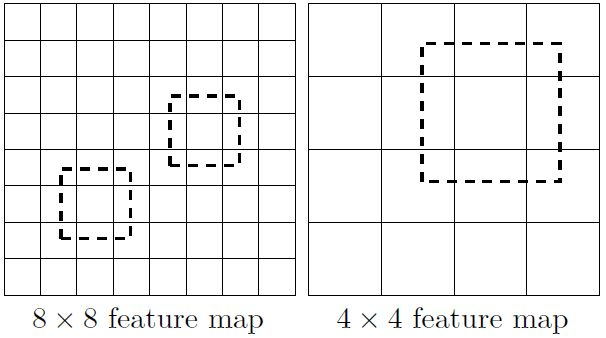
\includegraphics[width=\textwidth]{./Pictures/ssd_(2).jpg}	
	\caption{8x8与4x4的特征图}
	\label{featuremap}
\end{uscfigure}

\textbf{2、采用卷积进行检测}

与YOLO最后采用全连接层不同,SSD直接采用卷积对不同的特征图来进行提取检测结果。对于形状为 $m\times n \times p $的特征图,只需要采用$ 3\times 3 \times p $这样比较小的卷积核得到检测值。 

\textbf{3、设置先验框 }

在YOLO中,每个单元预测多个边界框,但是其都是相对这个单元本身(正方块),但是真实目标的形状是多变的,YOLO需要在训练过程中自适应目标的形状。而SSD借鉴了Faster R-CNN中anchor的理念,每个单元设置尺度或者长宽比不同的先验框,预测的边界框(bounding boxes)是以这些先验框为基准的,在一定程度上减少训练难度。一般情况下,每个单元会设置多个先验框,其尺度和长宽比存在差异,如图\ref{ssd_anchor}所示,可以看到每个单元使用了4个不同的先验框,图片中猫和狗分别采用最适合它们形状的先验框来进行训练,后面会详细讲解训练过程中的先验框匹配原则。
\begin{uscfigure}
	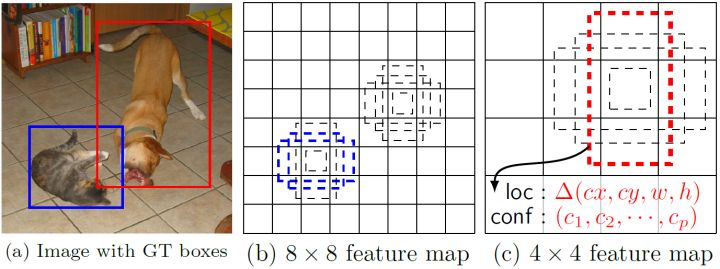
\includegraphics[width=\textwidth]{./Pictures/ssd_(3).jpg}	
	\caption{SSD算法中的先验框}
	\label{ssd_anchor}
\end{uscfigure}